% !Mode:: "TeX:UTF-8"
%!TEX program  = xelatex

%\documentclass{cumcmthesis}
\documentclass[withoutpreface,bwprint]{cumcmthesis} %去掉封面与编号页
\renewcommand{\arraystretch}{1}
\usepackage{url}
\usepackage{listings} 
\title{基于Mediachain的数字媒体知识产权交易系统}
\tihao{A}
%\baominghao{4321}
%\schoolname{XX大学}
%\membera{小米}
%\memberb{向左}
%\memberc{哈哈}
%\supervisor{老师}
%\yearinput{2017}
%\monthinput{08}
%\dayinput{22}

\begin{document}
 \maketitle
 \begin{abstract}
本文基于Mediachain数字媒体区块链管理技术建立IPTC知识产权交易模型,建立了易查询、易追溯的数字媒体分布式存储方式,实现了数字媒体版权的快速发布、分类授权和安全交易,从而实现了基于区块链的数字媒体版权收益分配,使发行方在交易系统中平等竞争,使用方在交易系统中得到快速授权,制作方在交易系统中便捷地明确收益。

在传统的中心化版权信息存储系统中,由于数字媒体有着对存储量需求巨大导致存储成本极高的特点,再加上数字媒体版权内容杂乱不易归类,使得中心化存储方案存储量较小,查询慢,对版权信息仅作形式审查,出现版权纠纷时法律支撑力度不够;这使得使用方和制作方信息不对称,各方之间的收益分配混乱。

本文提出的模型分成两部分:第一部分基于Mediachain实现了数字媒体版权的元数据和纲要分布式存储,借助IPFS分布式文件系统使数字媒体版权信息实现去中心化存储,使得数字媒体版权信息易归类易存储易交互。第二部分是IPTC数字媒体版权信息交易区块链,其中设立发行方、使用方和制作方三类用户,采取注册、交易、授权三种记录模式,DPoS共识机制和SPV快速支付机制,使交易信息不可变更地、独一无二地被记录在区块链上,之后根据区块链上交易信息的差异对各方进行收益分成。


\keywords{区块链\quad 知识产权\quad 去中心化}
\end{abstract}

%目录
\tableofcontents

\newpage

\section{问题重述}

\section{问题分析与背景介绍}
\subsection{问题分析}
分析一下题目要求与满足这些要求的模型类别——就是基于区块链的模型
\subsection{背景介绍}
这一部分主要想介绍一下已有的系统与模型。章节名可以另起。

\section{Mediachain元数据区块链模型}

\subsection{Mediachain模型综述}
Mediachain是美国Mediachain Labs公司开发的一种基于区块链技术的开源数字媒体版权保护机制。它的核心产品是一个元数据协议,通过它内容创作者可以给自己的作品附加信息,并把该数据打上时间戳放到对应的的区块链里,然后放到InterPlanetary File System(IPFS,吸收了区块链技术的分布式文件系统)上。其特点主要有如下几点:

(1)安全。Mediachain系统中的每个对象都是可寻址的和自我认证的,这意味着数据可以被多个不可信的参与者复制和使用,同时还能保持不可篡改性,因为数据完整性是通过加密认证的。

(2)可扩展。Mediachain规定了一个可扩展的元数据纲要(schema),使得数字媒体的元数据存储变得规范化并且调和不同的元数据,从而使对象之间的丰富关系可以用merkle DAGs表示。
这使得应用程序层可以根据用户的需求进行表达,且在系统中可以通过多种非破坏性的方式使用内容地址链接来引用或扩展数据。

(3)低成本。Mediachain采用点对点的去中心化的分布式数据库存储信息。所有数据都是定位的,任何人都能以安全的方式复制和服务他人的数据集,这降低了参与者的成本,并增加了访问数据时的带宽。

\begin{figure}[!h]
	\centering
	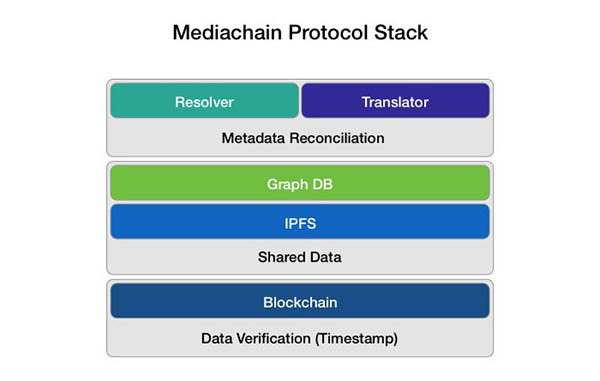
\includegraphics[width=.8\textwidth]{mediachain.jpg}
	\caption{Mediachain协议示意图}
\end{figure}

基于Mediachain的产权追溯流程如下:

step1: 数字版权所有者(一般是作者)加入区块链时,Mediachain会分配给版权所有者独一无二的Publisher ID(发布者ID),通过Publisher ID同时IPFS系统会通过非对称加密算法为版权所有者生成公钥和私匙,对公匙使用哈希方法生成peer地址。

step2: 当版权所有者想要发布数字媒体作品时,需要首先构建作品的声明信息,声明信息包括了指向作品元数据和纲要数据的索引,发行方的签名,时间戳,作品的分类,之后声明信息会随着加密货币被记录在区块链上,并且由时间戳构成防伪标志。这些声明信息会被记录员记录在区块链主链上,而作品的元数据则被发行方存储到自己的IPFS系统里。

step3: 版权所有者可以通过添加peer地址,之后使用Mediachain提供的合并机制把其他版权方的数字版权元数据合并到自己的IPFS分布式数据库里。网络上的peer地址里的元数据未必可信,这使得虽然有区块链主链保证声明的真实性,但直接访问整个IPFS网络会下载无意义的元数据,所以Mediachain允许使用者可以仅添加可信的peer地址来节约空间。

step4: 数字版权的使用者如果想使用这个数字作品,首先需要拥有数字作品的元数据,之后可搜索已添加的peer地址作为元数据库来源,使得使用者可通过作品元数据反向定位到声明以找到作者,并且在下文的产权交易模型中付费。至此,基于Mediachain数字媒体元数据区块链的产权追溯完成。

\subsection{Publisher ID的生成与Hash算法}
当Mediachain区块链主链上产生"发布声明"时,区块链上各记录员协调后生成的记录的有效性依赖于声明中的数字签名信息和用户对应的Publisher ID的准确性。模型中Publisher ID的构建依赖于hash算法。

\subsubsection{哈希表}

哈希表是根据关键码值(key)进行直接访问的数据结构。即将关键码值映射到表中一个位置来访问相应记录。如给出表M,确定函数f(key),对任意给定的关键字值key,代入函数后得到包含该关键字的记录在表中的地址(address),函数f(key)为即为表M的hash 函数。常见的哈希函数方法包括直接寻址法,数字分析法,随机数法等。

\begin{figure}[!h]
	\centering
	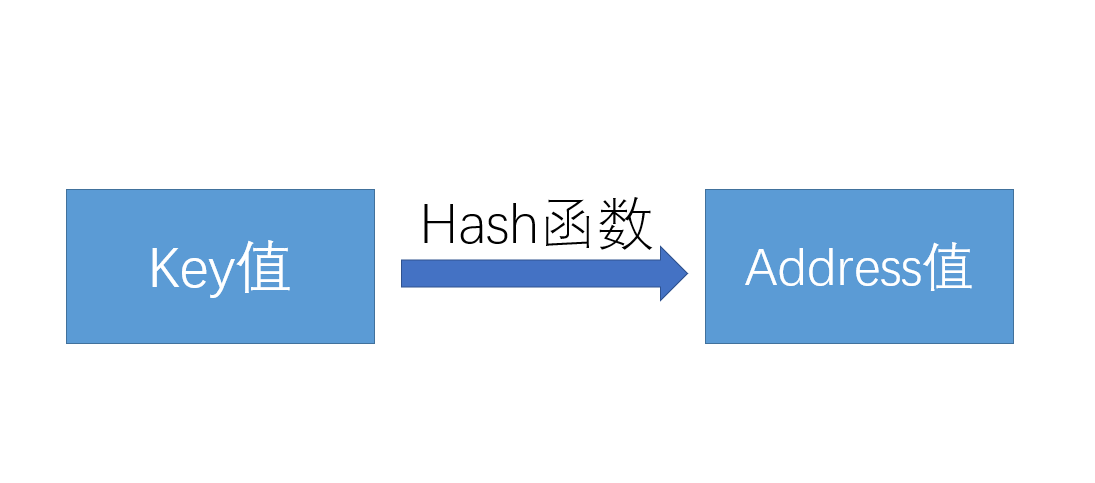
\includegraphics[width=.6\textwidth]{hash.png}
	\caption{hash映射}
\end{figure}

对不同的关键码值可能得到同一散列地址,即 $k1\neq k2$ ,而f(k1)=f(k2),这种现象称为碰撞(Collision)。具有相同函数值的关键字对该散列函数来说称为同义码值。这样的码值破坏了体系的一致性。这时,hash算法应该建立相应的防碰撞机制,例如开放寻址法和再散列法,建立另一个散列函数地址或建立探测散列的机制。同时,也可以加大哈希表的容量,从而增加伪造难度。

哈希表的优势首先在于不可逆性,由相应的地址很难得到对应的关键码值,这为安全性提供了有力的保障。同时,关键码值必须保证完全的准确性,暴力破解者很难完全建立正确的映射。

\subsubsection{SHA-256算法}

SHA-256 算法又称安全散列算法。其输入的最大长度不超过2*64 bit,输入按512-bit 分组进行处理,产生的输出是一个256-bit 的地址。该算法处理如下:

Step1 准备:

处理输入key的长度,使key长度满足mod 512 = 448,并将初始64位初始key值的位长度附加在后面。初始化缓存,使用一个256-bit 的8个缓存器来存放算法函数的中间及最终结果。 将处理后的512-bit(16个字)进行分组。

Step2运算:

使用基本的逻辑函数,进行迭代运算。可由分组之后的key值得到W(i)(i=0,1….15)再通过递推公式新的消息块W(i)(i=16,17….63).

SHA-256基于逻辑函数,每个函数均基于32位字运算,同样的这些函数的计算结果也是一个32位字。用缓存器缓存中间结果记作 ABCDEFGH,循环迭代下面公

$T_{i+1}=H_{i}+\sum_0{E_{i}}+Ch(E_{i},F_{i},G_{i})+K_{i}+W_{i}$

$T_{i+2}=\sum_1{A_{i}+Maj(A_{i}+B_{i}+C_{i})}$

$H_{i+1}=G_{i},G_{i+1}=F_{i},F_{i+1}=E_{i},E_{i+1}=D_{i}+T_{i+1}$

$D_{i+1}=C_{i},C_{i+1}=B_{i},B_{i+1}=A_{i},A_{i+1}=T_{i+1}+T_{i+2}$

W(i)的循环公式为

$W_{i}=W_{i-2}+W_{i-16}+\sum_a(W(i-15)+\sum_b(W(i-2)))$

上述逻辑函数定义如下

$CH( x, y, z) = (x\land y) \oplus  ( (x\land z)$

$Maj( x, y, z) = (x \land y) \oplus (x \land z) \oplus (y \land z)$

$\sum_0(x) = ROTR^{2}(x) \oplus ROTR^{13}(x) \oplus ROTR^{22}(x)$

$\sum_1(x) = ROTR^{6}(x) \oplus ROTR^{11}(x) \oplus ROTR^{25}(x)$

$\sum_a(x) = ROTR^{7}(x) \oplus ROTR^{18}(x) \oplus SHR^{3}(x)$

$\sum_b(x) = ROTR^{17}(x) \oplus ROTR^{19}(x) \oplus SHR^{10}(x)$

\begin{figure}[ht]
	\centering
	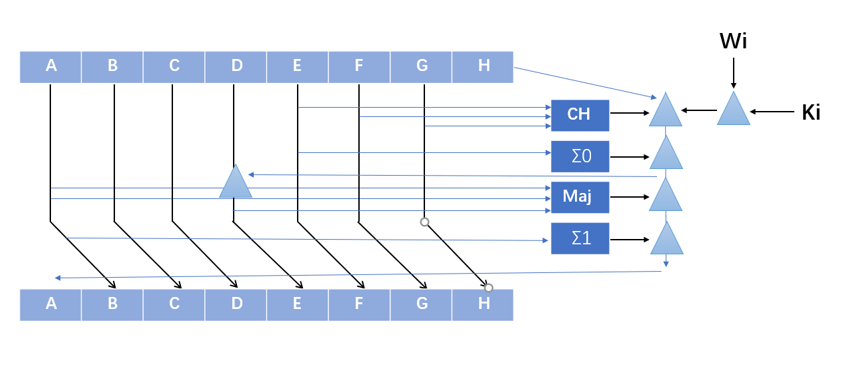
\includegraphics[width=.9\textwidth]{s256.png}
	\caption{SHA256流程图}
\end{figure}
Step3结果:

SHA-256算法最后一次缓存器存放结果产生的输出便是256-bit的address值。\newline

\subsubsection{公钥的生成--对应于Publisher ID}

1.每一个用户都要设置一个密码,由密码通过SHA256算法得到一个256位的数。通过ECC方法作用于这个数得到的码即为用户的公钥。

2.计算公钥的 SHA256 哈希值,并得到其结果的 RIPEMD160 哈希值。运算结束后在前面添加地址号得到前置地址。

注:RIPEMD (RACE Integrity Primitives Evaluation Message Digest,RACE原始完整性校验讯息摘要)是一种加密哈希函数。RIPEMD-160是以原始版RIPEMD所改进的160位元版本,而且是RIPEMD系列中最常见的版本。


3.两次计算 前置地址的 SHA-256 哈希值,取结果的后四个字节作为校验码。将校验码加在前置地址后面,即生成了用户地址的 16 进制结果。

4.将密码对应的sha-256值后面添加版本号(vis)和压缩标志(f)并在末尾添加校验码即生成私钥的 16 进制表示. 

\subsection{ECDH型数字签名}

整个版权交易与资金流通过程中,需要数字签名来建立一个认证机制。

模型中建立了基于椭圆曲线的ECDH数字签名的变体,设消息为m:

step1:签名生成

A.选择椭圆曲线,并确定相应基准点G

B.随机或伪随机的生成一个整数k属于$Z_n^*$,计算kG=(x1,y
1),r1=x1 mod n,r1=0,则

返回重选k

C.e=SHA-256(m)

D.r=r1e mod n,s=k + rd mod n,r=0或s=0,则重选k

step2:签名认证

A.接受者验证(r,s)是A对消息m的签名

B.验证r,s是[1,n-1]中整数

C.计算e=SHA-256(m)

D.X=sG-rQ=(x1,y1),X=0,拒绝这个签名,否则计算v=x1e mod n,只有v=r时认证成功。

\begin{figure}[ht]
	\centering
	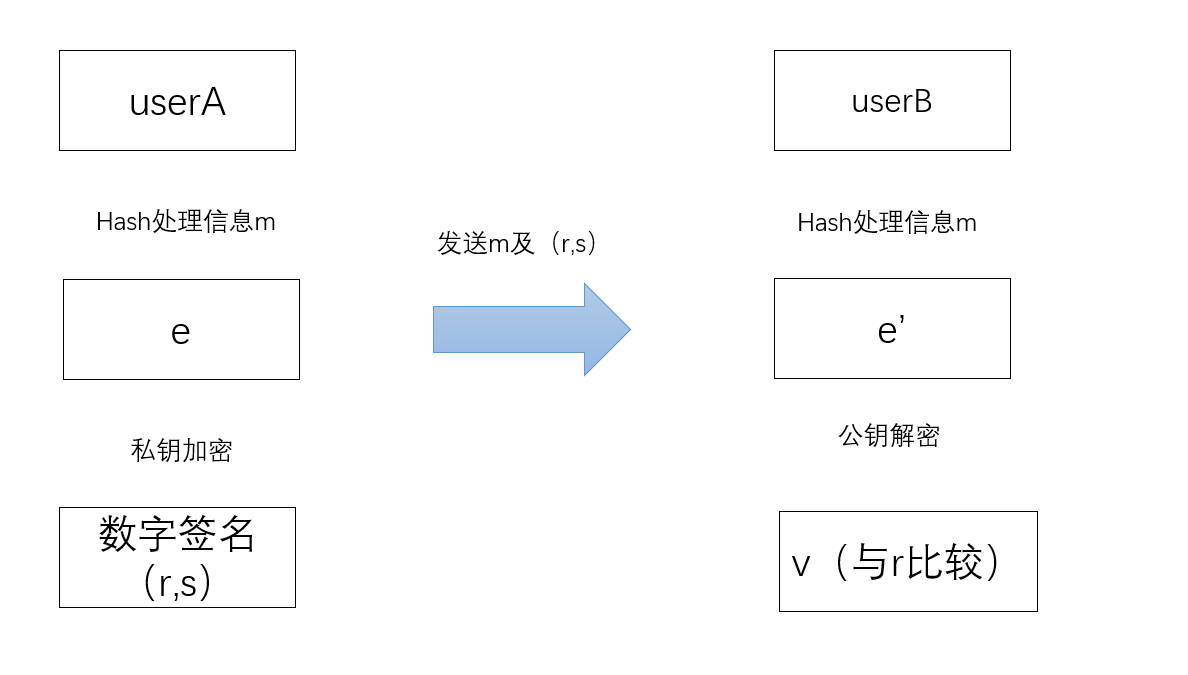
\includegraphics[width=.8\textwidth]{shu.png}
	\caption{数字签名认证}
\end{figure}

\subsection{Mediachain机制详解}
为了将数字作品版权加密存储在比特币区块链中,一般的做法是用OP\_RETURN或CoinSpark制作加密ID保存到区块链中,代表这些集中管理的数据;或者用定制的分布式账本将元数据直接绑定到每笔交易中。但这两种将元数据加密加入区块链的方法都有各自的缺点。比特币协议的OP\_RETURN内置代码每笔交易允许的最大数据容量是40字节,这样在区块链中存储更多元数据串就很难。于是,这种方法的效率就很低。第二个方法的缺陷在于其安全性。缺乏矿工和算力的新建网络对51\%攻击毫无抵抗力。一旦区块链和数据量扩展,保护数据安全的算力就更加紧张。

Mediachain并不依赖区块链的内置功能来存储元数据,采取了一种无需大量存储数据就可以验证数据的新方法,即通过声明来验证数据。

\begin{figure}[!h]
	\centering
	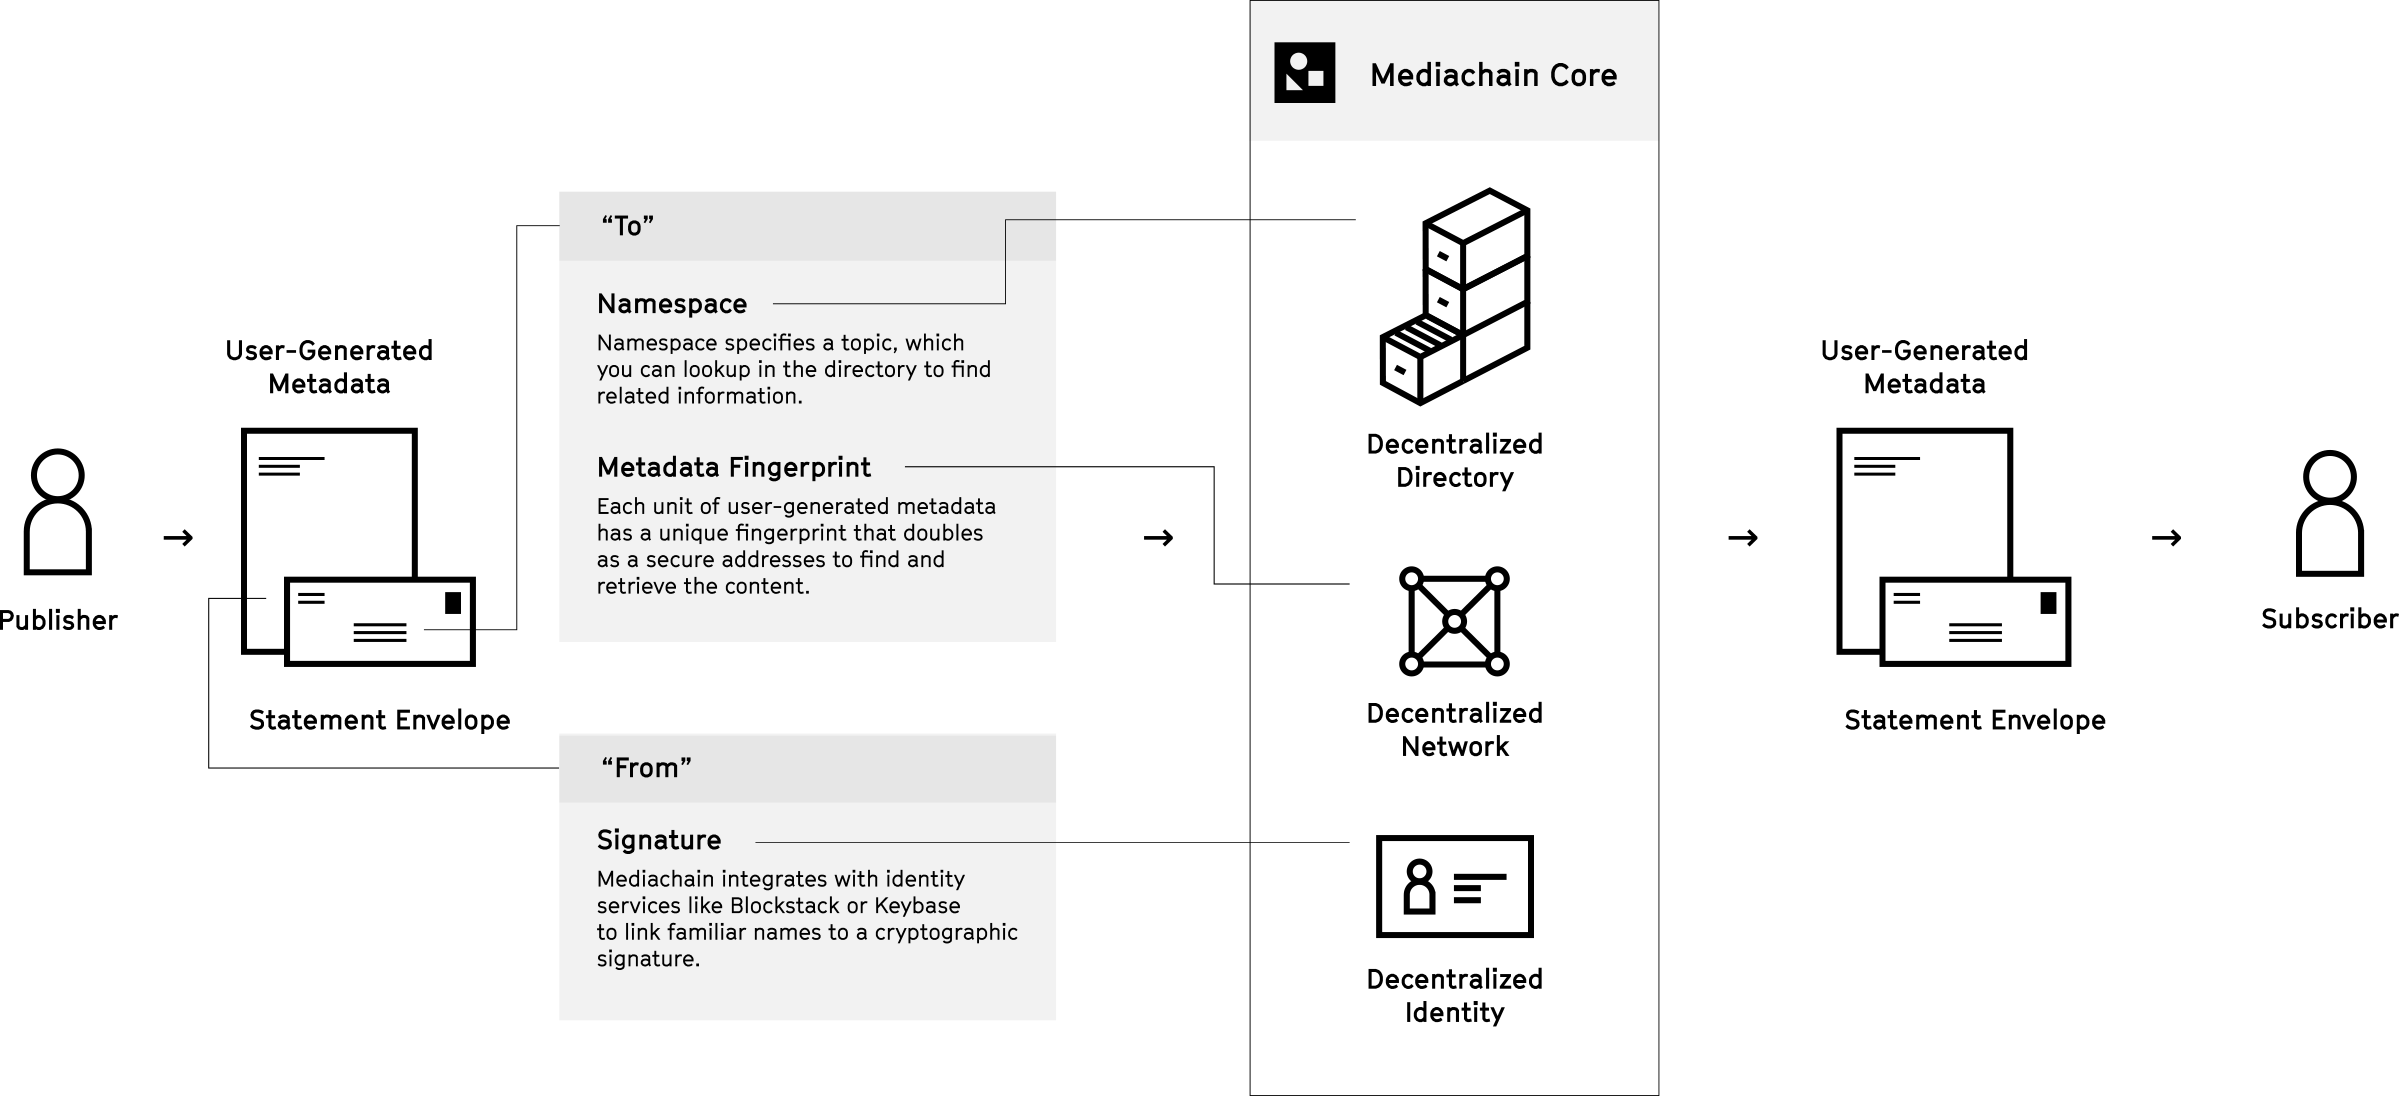
\includegraphics[width=.8\textwidth]{mc-stack.png}
	\caption{声明与元数据的关系类似于信封和信}
\end{figure}

在创建一个声明之前,必须先创建元数据文件,元数据文件包括了数字媒体作品的所有属性,包括创作时间,作者等等。之后还要创建元数据纲要文件,这个文件规定了上面提及的数字媒体属性分别是什么类别的,例如作者姓名是以字符串方式存储大小限制为8B,发表日期是以整数方式存储。作者在创建元数据文件和元数据纲要文件时均会使用SHA2-256算法生成唯一的哈希。命名空间则是一个独立的逻辑空间,使得Mediachain参与者不需要借助任何外部索引即可通过命名空间检索同类的作品版权声明,这使得IPFS系统中不同的参与者可以在同一个命名空间下协作。

声明(statements)包括如下信息:发布者ID,命名空间,元数据与纲要的哈希,数字签名,声明时间戳。这样产生的声明大小<40KB,可以存储到区块链里。接着按照比特币或以太坊提供的区块链防伪机制,以时间在最先的声明为真。以Moma博物馆对艺术作品的知识产权保护为例,有声明如下:

\begin{lstlisting}[language=C]
{
"id": "4XTTM7aPWTafN55cAwi882qnWy9XDv9EpGHU8rhPSYVA4yHaJ:1526090352:3", //声明ID
"publisher": "4XTTM7aPWTafN55cAwi882qnWy9XDv9EpGHU8rhPSYVA4yHaJ",  //发布者ID
"namespace": "museums.moma.artworks", //命名空间
"body": {
"simple": {
"object": "QmdFYwg17rdDV7qGm6jGTuYw3PBo2M25Fw84sp6etRJhjq", //元数据文件哈希
"refs": [
"moma:1"
],
"deps":"Qme1q1J2t2jpoaw21AbR2RUvTMVpqAavXGwrKeGu2ZFJuC"  //纲要文件哈希
}
},
"timestamp": "1526090352", //时间戳
"signature":   //数字签名
"B+OtKZ9J28g9gHYfF6w4NnSF+EtHLFfmEabXY2WctC4TcUeUXEDkM7ipPmYq48TxCzglgMe1C0b4aDQxZSS8AQ==" 
}

\end{lstlisting}


\subsection{IPFS分布式文件系统}

Mediachain采取IPFS文件系统存储数据,IPFS是一个开源分布式版本文件系统,它的目标是建立全球范围的点对点的文件传输。IPFS的原理是使用根据文件内容加密形成的哈希地址作为通讯地址,使用BitSwap协议传输,传输过程中只需验证文件的哈希是否正确而无需验证发送者的身份。对IPFS系统的详细介绍和可行性分析见后文第x节。


\section{IPTC知识产权交易模型}
\subsection{模型综述}
\subsubsection{记录与记录请求}
模型的基本思路是基于区块链思想,对知识产权的注册、授权等活动和与之相伴的资金流动以记录(transaction)的形式保存,并通过一定的机制保证其不可更改型与可信任性。从而实现对知识产权的注册、保护、使用与收益。

根据实际需要,记录分为以下三种:
\begin{description}
	\item[·注册记录] 在知识产权交易链模型中,知识产权的注册者、购买者与使用者等都应当是具有唯一ID的用户(user)。系统的使用者通过公布自己的ID与公钥而进入系统成为用户,此过程成为注册(register),而注册包含的信息则会被视为一条记录,其类型为注册记录(register transaction)。
	\item[·授权记录] 用于说明知识产权的授权、转移与使用等活动的记录是授权记录(authorization transaction)。在后面将会介绍,知识产权的注册是一条特殊的授权记录。
	\item[·支付记录] 而用户在为自己使用他人版权而付费时,需要向他人付款,付款相关信息的字符串是一条支付记录(payment transaction)。
\end{description}
记录的格式会在第2节详细说明。

在记录的提供者将记录内容准备好后,将记录向全网进行广播(实际上只需要向全部的服务商进行广播),被视为发出了记录请求(transaction request)。记录请求将会进入请求缓存区域(TRB,transaction request buffer),等待被被服务商添加至IPTC。

\subsubsection{服务商}
在传统的区块链系统中,所有的用户都具有创造区块的权力,而为争夺这种权力,经典的PoW(Proof of
 Work)共识机制需要付出大量不必要的额外的算力成本。但在知识产权系统中,希望利用的是区块链区去中心化、去信任、集体维护、记录可靠性等特性,而不希望浪费大量的算力在工作量证明上。同时,在分布式文件存储系统中(在本模型中为IPFS),每个系统的节点都有提供文件存储的义务。但注册与使用知识产权的大部分用户的关注点本身在与知识产权,仅希望获得服务而不希望提供存储与计算义务。
 
针对这些问题,模型提供了一类特殊用户,为其他用户提供必需的服务,被称为服务商(server)。服务商取代了传统知识产权体系中发行商的角色。

服务商提供的服务主要有:
\begin{description}
	\item[·有效性检验服务] 因为TRB内的记录请求可能存在签名不匹配,用户注册时用户ID重复,授权时授权人不具有授权资格,版权注册时作品已被注册,交易时账户余额不足等一系列问题导致记录为无效记录。因此需要对TRB中的记录作有效性检验,只有有效的记录才有可能被添加到IPTC中。检验时需要对IPTC进行搜索,计算工作量较为庞大,因此由服务商提供。有效性验证将在第3节详细说明。
	\item[·存储服务] 服务商首先应当存储全部的IPTC链。同时系统中注册的全部作品的存储应由服务商通过IPFS分担,并由BitSwap机制保证公平性。IPFS将会在第4节详细说明。
	\item[·记录服务] 只有服务商有权将记录添加至IPTC,减少了计算难度,提高了记录效率。通过DPoS共识机制保证其去中心化的特性。该机制将会在第5节详细说明。
\end{description}

类似于发行商,服务商会因为提供这些服务而盈利。举例说明,例如创作者为自己的作品注册,则A首先提交作品的备份至IPFS,在BitSwap机制下确定服务商为之提供存储服务,则A的版权收入会按比例抽取一小部分支付给提供这些服务商。之后A发出注册版权的记录请求,在DPoS共识下由服务商S为其提供有效性检验服务与记录服务,则服务商S也会从中按比例抽取一小部分作为服务费用。又如A向B支付一定金额的电子货币,则负责记录这条支付记录的服务商也会从中抽取一部分,作为服务费。

\subsubsection{区块创建与添加}
通过DPoS共识选出的见证人服务商向IPTC中不断添加新的区块。本部分内容将在第6节详细说明。

\subsubsection{用户端}
用户端是用户使用系统功能的窗口。在实际应用中,用户可以不必知道自己交易发生的具体细节,仅需提供操作的必要信息,由用户端为其执行具体操作,大致可以分为:
\begin{description}
	\item[·IPFS文件的上传与下载] 制作者通过用户端同时提交自己的作品和作品元数据元数据至Mediachain IPFS,并返回作品的MediachainID;使用者在获得授权之后通过用户端从IPFS下载作品。
	\item[·生成并提交记录请求] 在用户提供了用户ID、作品ID或是交易金额等必要信息之后,由用户端生成相应格式的记录并自动生成签名,提交至TRB。
	\item[·选举见证人] 用户通过用户端在DPoS中为自己新任的见证人投票。
	\item[·查询IPTC并整合信息] 在很多时候,用户需要对IPTC中的信息进行查询并整合,例如账户余额、自己作品的授权情况,自己的创意是否已经在IPFS中存在,支付是否完成等等。因此用户端也需要提供这些功能。SPV(Simplified Payment Verification,简单支付验证)被应用于此处以提高效率。该方法将在第7节详细说明。
\end{description}


SPV是“Simplified Payment Verification”(简单支付验证)的缩写。中本聪论文简要地提及了这一概念,指出:不运行完全节点也可验证支付,用户只需要保存所有的block header就可以了。用户虽然不能自己验证交易,但如果能够从区块链的某处找到相符的交易,他就可以知道网络已经认可了这笔交易,而且得到了网络的多少个确认。

\subsubsection{模型概览}
首先由用户根据需求与共识,创建记录。并通过用户端将记录请求提交至记录缓冲区,向全部服务商广播。根据DPoS共识在服务商中进行见证人选举,确定一位服务商对记录请求进行有效性检验,并将检验通过的记录打包创建区块,在自己的记录时间到来时根据已有的IPTC链将区块添加,并将新链广播。同时,用户可以通过用户端对IPTC链与IPFS进行目标信息的查询。

整个模型的流程如下图。
%\newpage
\begin{figure}[h]
	\centering
	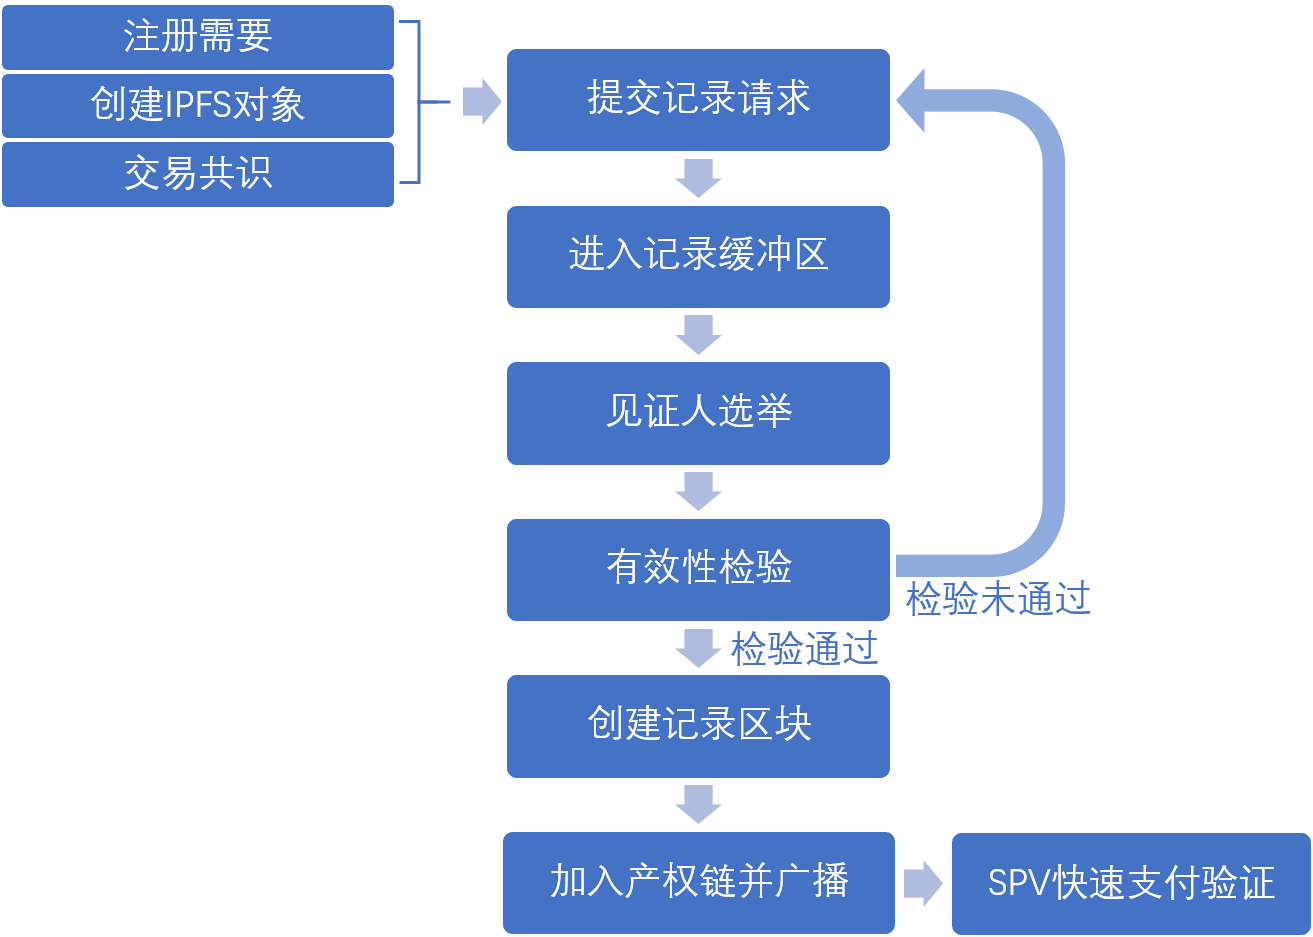
\includegraphics[width=.6\textwidth]{soo1.png}
	\caption{IPTC模型流程图}
\end{figure}
\begin{figure}[h]
	\centering
	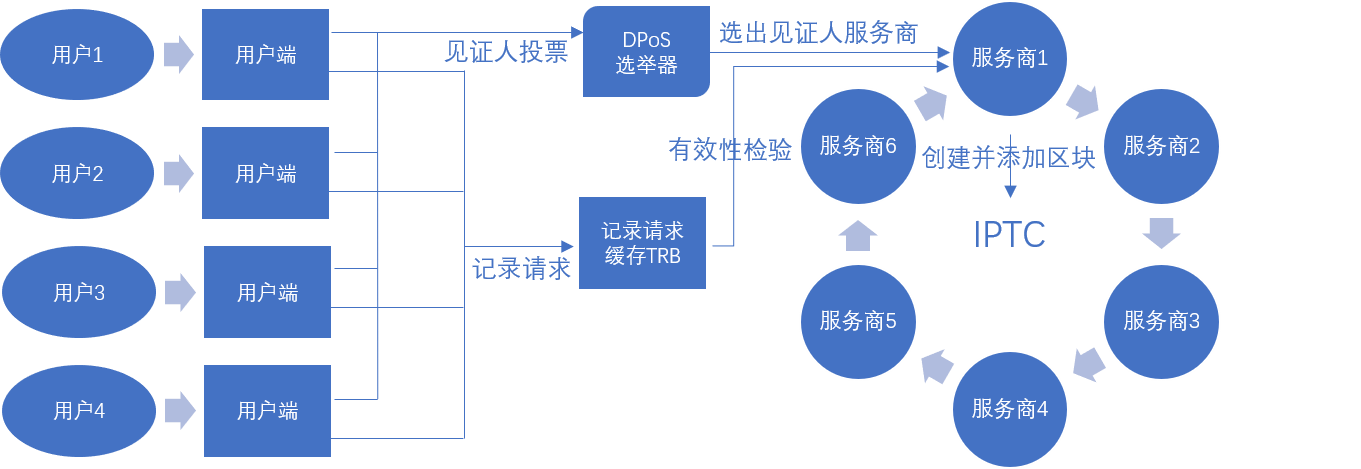
\includegraphics[width=\textwidth]{soo2.png}
	\caption{IPTC模型结构}
\end{figure}
\begin{figure}[h]
	\centering
	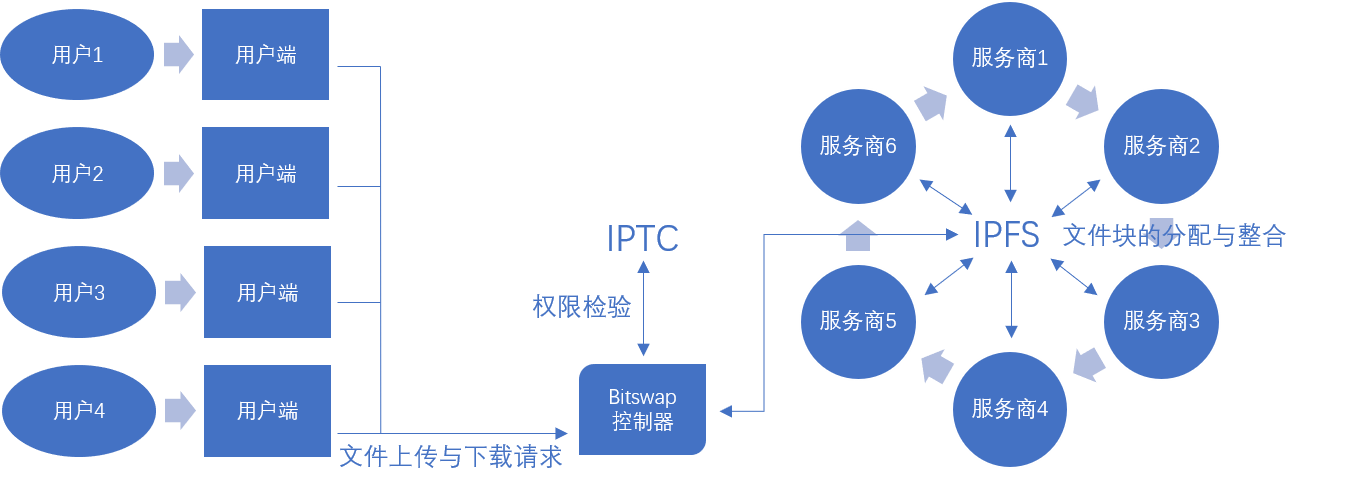
\includegraphics[width=\textwidth]{soo3.png}
	\caption{IPFS模型结构}
\end{figure}
\begin{figure}[h]
	\centering
	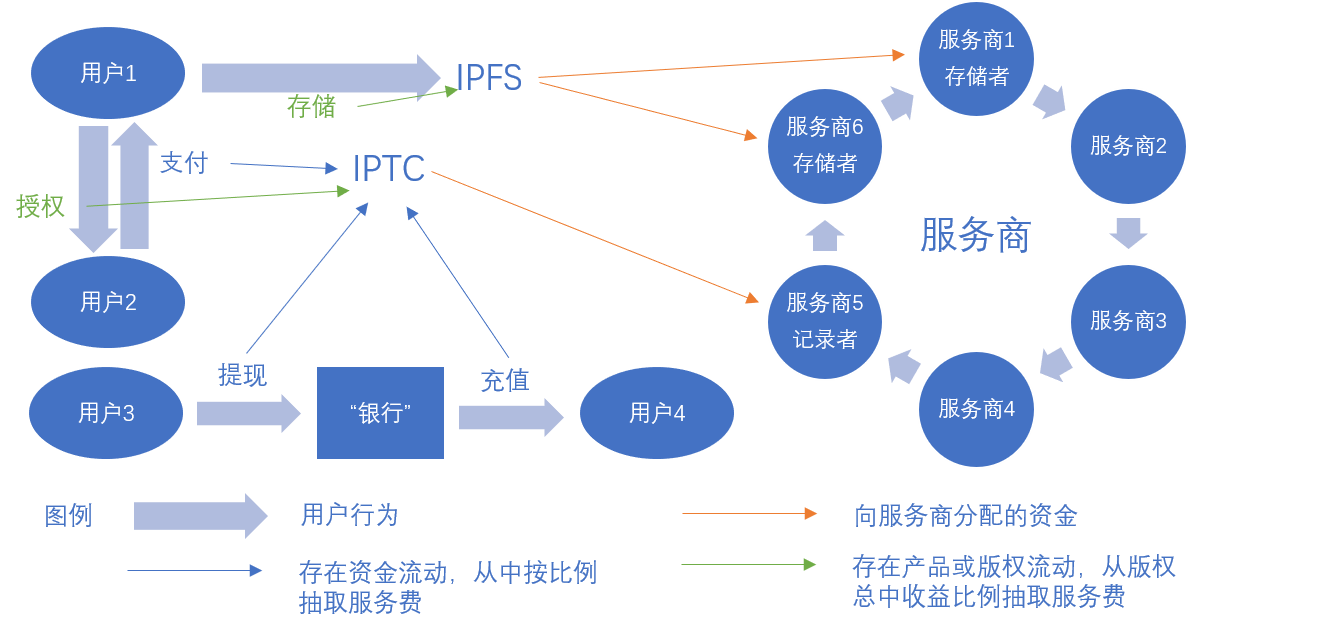
\includegraphics[width=\textwidth]{soo4.png}
	\caption{服务费示意}
\end{figure}

\subsection{记录生成}
三种记录的格式具体如下:
\[transaction\_type||content||timestamp||sinature\]
记录类型分别为第1节中描述的三种,记录内容为每种类型需要的必要信息。时间戳用于保证即使是类型与内容完全相同的记录也得到完全不同的hash,数字签名用于验证记录的可信性。

\subsubsection{注册记录(RT)}
\begin{description}
	\item[·记录类型] 注册记录(register transaction)。
	\item[·记录内容] $user\_id || public\_key$
	\item[·数字签名] 无须数字签名
\end{description}
在知识产权交易链模型中,知识产权的注册者、购买者与使用者等都应当是具有唯一ID的用户(user)。RT的作用即表明系统中用户的存在与相关信息。使用者通过RT来声明用户ID与公布公钥。当RT被成功添加进入IPTC中时,注册生效。在进行用户ID检索或者公钥查询时,在IPTC中搜索相应的注册记录,获得相应信息。


\subsubsection{授权记录(AT)}
\begin{description}
	\item[·记录类型] 授权记录(authorization transaction)。
	\item[·记录内容] $mediachain\_id || author\_id || licensee\_id || authorization\_type$
	\item[·数字签名] 作者的数字签名
\end{description}

注册人在向他人授权使用自己的作品时,需要公布作品ID与授权人被授权人的用户ID已经授权方式(例如授权使用、授权出售、产权转移等)并附有自己的数字签名确保其有效性,这些信息构成AT。当AT所在区块被加入IPTC时,授权生效。

在用户在为自己的新创作注册版权时,应当首先为自己的作品和作品元数据建立IPFS对象,为了节约空间,我们将作品元数据对应的MediachainID即作品ID。创作人将作品ID,用户ID公布并提出想要成为作品版权所有者的请求。这是一条特殊的AT,授权人与被授权人都为该用户,并且授权方式为“作者(author)”。

\subsubsection{支付记录(PT)}
\begin{description}
	\item[·记录类型] 支付记录(payment transaction)。
	\item[·记录内容] $amount\_of
	\_money || payer\_id || payee\_id$ 
	\item[·数字签名] 付款人的数字签名
\end{description}

而用户在为自己使用他人版权而付费时,需要向他人付款。同样的,付款人须公布支付金额、付款人ID与收款人ID,并附有自己的数字签名确保其有效性,这些信息构成PT。当PT所在区块被加入IPTC时,支付生效。

需要注意的是,因为系统中存在资金的流通,因此需要一定的数字货币作支撑。但考虑到知识产权交易链中的主要目的为知识产权的保护与交易,因此不应当设置独立的货币体系,而应当由权威的金融机构保证系统中数字货币与现实中流通货币汇率的固定性。因此需要一特殊用户“银行(Bank)”。用户首先在现实中向“银行”转账而获得系统中“银行”向用户的付款从而获得系统中的电子货币。同样,版权人如果希望将账户上的余额提现,应当向“银行”用户付款,进而在现实中从“银行”提现。在模型的实际应用中,“银行”用户的角色可以由一个信用良好的银行来承担。

\subsection{有效性检验}
如概览所述,可能在TRB中的记录请求可能是恶意伪造或是无效的,需要首先对其进行有效性检验。对于通过检验的记录,打包为区块加入IPTC;对于没有通过检验的记录,驳回请求(reject)并告知利益相关用户本次异常。对于不同类型的记录,有效性检验分别如下。
\subsubsection{注册记录(RT)}
在IPTC中搜索$user\_id$,如果找到则为无效记录,驳回请求;否则视为有效记录将记录,打包入区块。
\\

\fbox{\shortstack[l]{
\textit{\% register transaction validation}\\
{\bfseries function} register\_transaction\_validation($transction$) \\
\quad $transction$ \ = \ $transaction\_type||content||timestamp||sinature$\\
\quad $content$ \ = \ $user\_id || public\_key$\\
\quad {\bfseries if} $user\_id$ {\bfseries in} IPTC.userIDs()\\
\quad \quad transaction\_reject()\\
\quad \quad inform($user\_id$, \ USERIDCONFLICT)\\
\quad {\bfseries else}\\
\quad \quad pack\_transaction($transction$)\\
\quad {\bfseries end if}\\
\quad {\bfseries return}\\
{\bfseries end function}
}}

\subsubsection{授权记录(AT)}
如果是版权注册,则授权人与被授权人相同。在IPFS中搜索 $mediachain\_id$的作者信息,若校验失败,驳回请求并告知原作者与注册人;否则视为有效记录将记录,打包入区块。

否则为授权活动,首先验证签名有效性,若签名无效,驳回请求并警告作者与被授权人。如果签名有效,进一步验证$author\_id$是否有授权资格,如果没有,驳回请求并则告知双方;否则视为有效记录将记录,打包入区块。
\\

\fbox{\shortstack[l]{
\textit{\% authorization transaction validation}\\
{\bfseries function} authorization\_transaction\_validation($trasaction$) \\
\quad $trasaction$ \ = \ $transaction\_type||content||timestamp||sinature$\\
\quad $content$ \ = \ $ipfs\_id || author\_id || licensee\_id || authorization\_type$\\
\quad {\bfseries if} $author\_id$ == $licensee\_id$\\
\quad \quad {\bfseries if} $user\_id$ {\bfseries in} IPTC.userIDs()\\
\quad \quad \quad transaction\_reject()\\
\quad \quad \quad inform(IPTC.authorIDs($ipfs\_id$), \ $author\_id$, \ WORKSREGISTERED)\\
\quad \quad {\bfseries else}\\
\quad \quad \quad pack\_transaction($transction$)\\
\quad \quad {\bfseries end if}\\
\quad \quad {\bfseries return}\\
\quad {\bfseries end if}\\
\quad {\bfseries if} check($transaction$,\ $signature$,\ get\_pk($author\_id$))\\
\quad \quad {\bfseries if} $author\_id$ {\bfseries in} IPTC.authorID($ipfs\_id$)\\
\quad \quad \quad pack\_transaction($transction$)\\
\quad \quad {\bfseries else}\\
\quad \quad \quad transaction\_reject()\\
\quad \quad \quad inform($author\_id$,\ $licensee\_id$,\ NOAUTHORITY)\\
\quad \quad {\bfseries end if}\\
\quad {\bfseries else}\\
\quad \quad transaction\_reject()\\
\quad \quad inform(IPTC.authorID($ipfs\_id$), \ $licensee\_id$, \ FALSESIGNATURE)\\
\quad {\bfseries return}\\
\quad {\bfseries end if}\\
{\bfseries end function}
}}

\subsubsection{支付记录(PT)}
首先验证签名有效性,若签名无效,驳回请求并警告付款人与收款人。如果签名有效,进一步验证$payer\_id$余额是否足以完成本次支付,如果不能,驳回请求并则告知双方;否则视为有效记录将记录,打包入区块。
\\

\fbox{\shortstack[l]{
	\textit{\% payment transaction validation}\\
		{\bfseries function} payment\_transaction\_validation($trasaction$) \\
		\quad $trasaction$ \ = \ $transaction\_type||content||timestamp||sinature$\\
		\quad $content$ \ = \ $amount\_of
		\_money || payer\_id || payee\_id$\\
		\quad {\bfseries if} check($transaction$,\ $signature$,\ get\_pk($payer\_id$))\\
		\quad \quad {\bfseries if} IPTC.afford($payer\_id$,\ $amount\_of
		\_money$)\\
		\quad \quad \quad pack\_transaction($transction$)\\
		\quad \quad {\bfseries else}\\
		\quad \quad \quad transaction\_reject()\\
		\quad \quad \quad inform($payer\_id$,\ $payee\_id$,\ INSUFFICIENTFUNDS)\\
		\quad \quad {\bfseries end if}\\
		\quad {\bfseries else}\\
		\quad \quad transaction\_reject()\\
		\quad \quad inform($payer\_id$, \ $payee\_id$, \ FALSESIGNATURE)\\
		\quad {\bfseries return}\\
		\quad {\bfseries end if}\\
		{\bfseries end function}
}}



\subsection{IPFS分布式文件存储系统}

IPFS是一个开源分布式版本文件系统,它的目标是建立全球范围的点对点的文件传输。IPFS的原理是使用根据文件内容加密形成的哈希地址作为通讯地址,传输过程中只需验证文件的哈希是否正确而无需验证发送者的身份。

IPFS让应用可以完全控制对象的数据字段,即可以随意定义对象的data类型和结构,灵活度非常大。IPFS数据对象格式如下:
\begin{lstlisting}[language=c]
type IPFSLink struct {
Name string             // link 的名字
Hash Multihash        // 数据的加密哈希
Size int                    // 数据大小
}
Type IPFSObject struct {
links []IPFSLink        // link数组
data []byte               // 数据内容
}

\end{lstlisting}
其中,IPFS对象的data段是不超过256KB的任意数据,每个IPFS对象可能被分发到不同的计算机上存储,通过Merkle有向无环图进行检索与合并。

\subsubsection{Merkle有向无环图}

Merkle有向无环图(Merkle DAG)是IPFS使用的基本数据结构,它与Merkle树十分相似。Merkle树是一种叶子节点被数据块的哈希标记,非叶子节点被子节点的加密哈希所标记的树。Merkle树允许在叶子节点把数据分成小的数据块,有相应的哈希值与之对应,在非叶子节点将相邻的两个哈希合并,由合并字符串生成新的哈希。于是在树根只有一个哈希,这个哈希就是根哈希,在进行p2p网络下载前只需从可信源获得根哈希,即可从其他不可信的源获取Merkle树节点,并进行分支验证,若生成的根哈希与取得的相同,则说明内容无误。如果Merkle树是损坏的或者虚假的,就从其他源获得另一个Merkle树,直到获得一个与可信树根匹配的Merkle树。

\begin{figure}[!h]
	\centering
	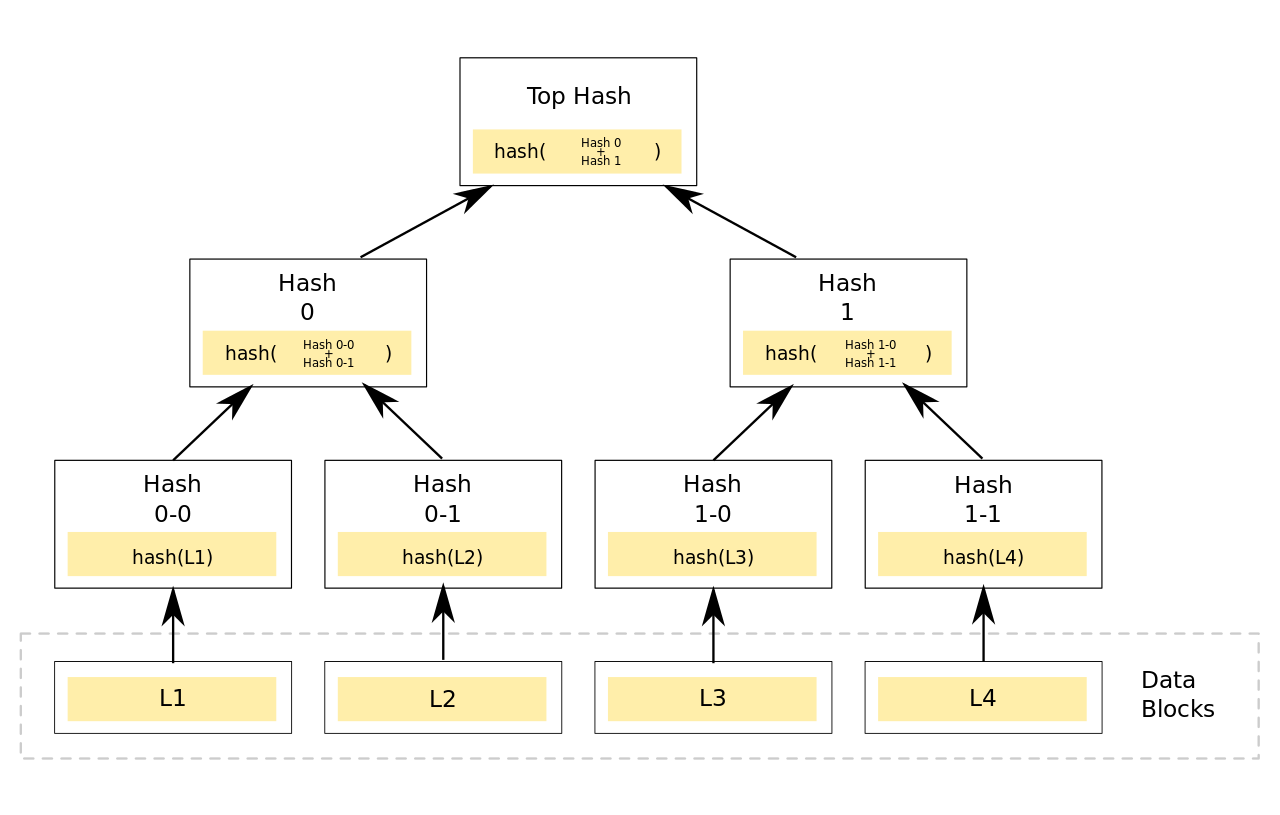
\includegraphics[width=.8\textwidth]{logo-108.png}
	\caption{Merkle树示意图}
\end{figure}

Merkle DAG的主要特点是可以在非叶子节点存储数据,并且不需要进行树的平衡操作。此外,树在面临子树重复出现时浪费了存储空间,此时使用DAG可以实现对相同子树的共享。Merkle DAG相关操作有创建、更新、插入、删除、遍历,算法上与普通有向无环图的操作一致,可以使用深度优先搜索和广度优先搜索进行遍历,故不赘述。下面以在IPFS系统中创建数字媒体作品为例展示算法流程:

step1: 对数字媒体作品切块处理,之后对数据块做hash运算,$Node_{0i}=hash(Data_{0i}),i=1,2,3,...,n,j=1$

step2:相邻两个hash块串联,然后做hash运算,$Node_{j(\frac{i+1}{2})}=hash(Node_{(j-1)i}+Node_{(j-1)(i+1)})$

step3: $j=j+1$,重复step2,直至得到根节点为止

step4:得到根节点,Merkle DAG生成完毕,算法复杂度为$O(n)$,最小生成树的长度为$log(n)+1$。

IPFS主要使用Merkle DAG进行文件存储。它将文件分成若干小块,每个块被赋予唯一的加密哈希。Markle DAG通过合并子树可以删除具有相同哈希值的节点,并跟踪每个文件的版本历史记录。查找文件时,通过文件的哈希值就可以在网络查找到储存该文件块的节点,找到想要的文件。

\subsubsection{BitSwap数据传输协议}
IPFS系统不仅包括文件存储,它在BitTorrent的基础上实现了p2p数据交换协议BitSwap。跟BitTorrent不一样的是:BitSwap获取数据块的时候不限于同一个torrent。从全局考虑,这使得BitSwap的效率更高。

为鼓励节点多分享数据,BitSwap提出信用体系:(1)节点记录自己与其他节点的传输平衡状况;(2)节点传输给负债节点数据的概率随负债的增加而减少。信用体系因不同的传输对象而异,在本模型中,为了同时保证数字媒体资源具有较高的下载速度,取BitSwap负债率的定义如下:

\[ 
r=\sqrt{\dfrac{|\dfrac{bytes\_sent}{1G}|}{|\dfrac{bytes\_recv}{1G}|+1}}
\]
\[
P(send|r) = 0.8*(1 - \dfrac{1}{1+e^{6-3r}})+0.2 
\]

其中$byte\_sent$为该节点发送的数据,$byte\_recv$为该节点接受的数据,r为负债率,$P(send|r)$为负债率为r时发送数据给该节点的概率。

\begin{figure}[!h]
	\centering
	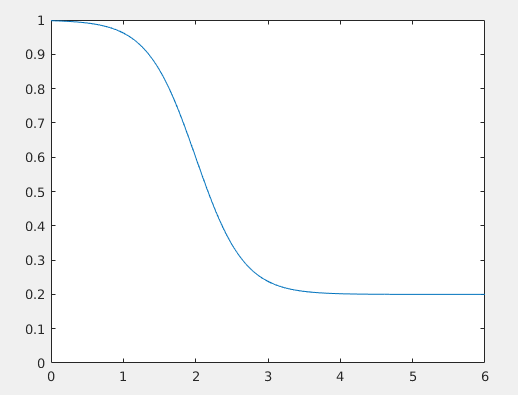
\includegraphics[width=.5\textwidth]{untitled.png}
	\caption{发送率随负债率变化曲线}
\end{figure}

如果把IPFS用户打开默认的上传功能,且仅仅上传刚接收到的数据,则$r\equiv1$,数据发送率高于90\%,如果继续转发接受的数据,则数据发送率将达到95\%以上,系统是稳定的。若节点上传接受数据的1/4则可以保持80\%的下载速度。若IPFS节点一直拒绝发送,则累计下载4G文件后下载速度减半,累计下载9G文件后没有下载加成,下载速度只有全网的20\%。

\subsubsection{可行性分析}

由于传播数字媒体时往往伴随着较高的下载量和较低的上传量,故在本模型中上传是一种被奖励的行为,奖品是更高的下载速度,而不是原BitSwap协议中要求的必需品。同时去中心化的Merkle DAG存储模式节约了大量的储存空间并且整合利用了闲置资源,这符合现代数字媒体体积大下载量高的特点,同时,Merkle DAG模式使得完整的数字媒体以碎片化的形式保存到第三方服务器上,更安全地保护了数字媒体版权,故采用IPFS系统存储数字媒体是可行的。

\subsection{DPoS共识机制}
为实现IPTC的去中心化,应当有一套全部用户可以达成共识的共识机制来决定创建区块与并添加至IPTC的用户。比特币系统采用的是PoW(Proof of Work,工作量证明)共识机制。这种机制的出发点是希望区块链中所有节点在算力足够的前提下都可以有机会通过进行记录操作。但是这种共识机制浪费了大量的算力与电力资源,这与系统的初衷:对知识产权实现快速的记录、授权与交易的目的是相悖的。而且现在许多拥有庞大算力资源的矿池基本集中了对比特币的控制,与“去中心化”的特性背道而驰。

因此在IPTC中,采用了另一种共识机制DPoS(Delegated Proof of Stake,股份授权证明机制)。该机制通过全体用户投票,票数最高的一定数量的用户作为见证人,进行区块操作。考虑到IPTC模型中并不是所有用户均有希望通过区块操作盈利,而将有此类需求的用户列为服务商,所有用户在服务商中投票。达到一定票数与比例要求的服务商轮流完成区块操作。





101位




\subsection{IPTC区块生成}


在IPTC区块链中,数据会以文件的形式被永久记录,我们称这些文件为区块。一个区块是一些或所有最新知识产权交易的记录集,且未被其他先前的区块记录。新区块会被加入到记录的最后,一旦写上,就再也不能改变和删除。每个区块记录了它被创建之前发生的所有事件。一个完整的IPTC区块由下面几部分组成:区块头,区块大小,交易计数器和交易(区块主体)。

\begin{figure}[!h]
	\centering
	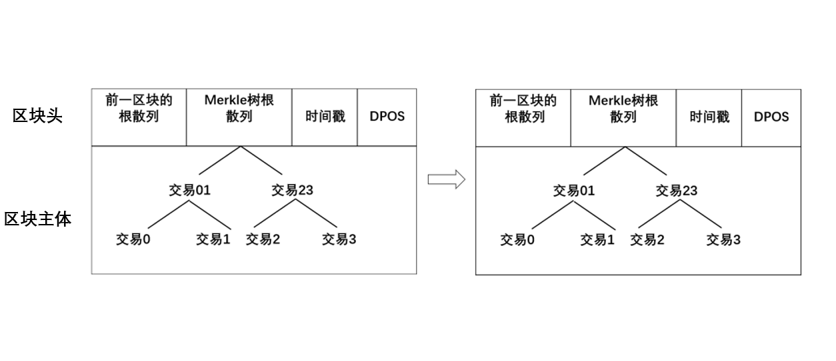
\includegraphics[width=1\textwidth]{IPTC.png}
	\caption{IPTC区块在时间上的分布}
\end{figure}

\begin{table}[h]
	\caption{IPTC区块组成结构}\label{tab001} \centering
	\begin{tabular}{ccc}
		\toprule[1.5pt]
		字节 & 字段 & 说明 \\
		\midrule[1pt]
		4 & 区块大小 & 用字节表示的该字段之后的区块大小\\
		80 & 区块头 & 组成区块头的几个字段\\
		1-9 & 交易计数器 & 该区块包含的知识产权交易数量\\
		不定 & 交易 & 记录在区块里的交易信息,使用知识产权交易信息格式,\\
		& & 分为RT、AT和PT,并且交易在数据流中的位置\\
		& & 必须与Merkle树的叶子节点顺序一致\\
		\bottomrule[1.5pt]
	\end{tabular}
\end{table}
IPTC的区块大小目前被严格限制在1MB以内,其中4字节的区块大小字段不包含在此内。

\newpage

\begin{table}[h]
	\caption{IPTC区块头结构}\label{tab001} \centering
	\begin{tabular}{ccc}
		\toprule[1.5pt]
		字节 & 字段 & 说明 \\
		\midrule[1pt]
		4 & 版本 & 区块版本号,表示本区块遵守的验证规则\\
		32 & 父区块头哈希值 & 前一区块的哈希值,使用SHA256(SHA256(父区块头))计算\\
		32 & Merkle根 & 该区块中交易的Merkle树根的哈希值,\\
		& & 同样采用SHA256(SHA256())计算\\
		4 & 时间戳 & 该区块产生的近似时间,精确到秒的UNIX时间戳\\
		4 & 难度目标 & 该区块工作量证明算法的难度目标,由DPoS机制决定\\
		\bottomrule[1.5pt]
	\end{tabular}
\end{table}
IPTC区块头中,版本信息、父区块头哈希值和Merkle根采用的是小端格式编码,即低有效位放在前面。
时间戳表示的是自1970年1月1日0时0分0秒以来的秒数,1231731025秒转为十六进制值为0x496AB951,然后采用小端格式编码表示为0x51b96a49。IPTC区块主体由众多交易组成,每一笔交易结构如下:

\begin{table}[h]
	\caption{IPTC区块交易结构}\label{tab001} \centering
	\begin{tabular}{ccc}
		\toprule[1.5pt]
		字节 & 字段 & 说明 \\
		\midrule[1pt]
		4 & 交易ID & 用于定位交易\\
		4 & 交易类型 & 用于决定采用何种交易记录方式\\
		32 & MediachainID & 作品在IPFS中的哈希\\
		32 & userID & 用户的哈希\\
		32 & pubKey & 用户的公匙(注册时出现)\\
		32 & publisherID & 发行商的哈希\\
		32 & payID & 付款方的哈希\\
		32 & recvID & 收款方的哈希\\
		4 & 授权类型 & 有A,B,C三种用于区分授权\\
		4 & Payment & 付款的数额\\ 
		32 & paySign & 付款方的签名\\
		32 & recvSign & 收款方的签名\\
		32 & paySign & 付款方的签名\\
		32 & Signature & 版权方的签名\\
		4 & 时间戳 & 该区块产生的近似时间,精确到秒的UNIX时间戳\\
		64 & Merkle索引 & 用于确定交易所处与的Merkle树位置\\
		\bottomrule[1.5pt]
	\end{tabular}
\end{table}

\subsection{SPV快速支付验证}
在用户使用IPTC时,需要通过用户端检索自己需要的信息。例如自己作品授权情况,自己的账户余额,一笔交易有没有完成等等。而获取这些信息往往需要极大的搜索工作量。一方面,可以令用户端记录由用户发出的所有记录请求。而对于其他用户发出的,以自己为目标的记录,可以通过SPV快速验证。SPV(Simplified Payment Verification),即简单支付验证。使用这一概念极大地减轻了用户交易记录的负担。

\subsubsection{两种验证方式}

在版权授权过程中,创作者P收到来自请求授权者U的通知,U声称已经从某账户将资金转移给了P。去中心的区块链系统中,这一通知包含在固定格式的交易记录中。

P如果想要验证这笔交易的真实性,需要遍历完整的区块链记录账本。首先定位U的账户并检查资金是否充足,然后遍历其后续记录查看是否存在双花欺骗,还要验证U对账户的支配权。这个过程非常复杂,且需消耗大量存储空间。

因此,可抛开交易,确定资金转移是否被验证,并得到多少算力保护,即SPV方法。

\subsubsection{基于block header的SPV}
	
无论交易量有多大,block header(区块头)的大小始终只有80字节。其中含有三个关键字段,一是prev\underline{\hspace{0.5em}}block\underline{\hspace{0.5em}}hash(前一区块的hash值,确保了区块链所记录的交易次序);二是bits(当前区块的计算难度), 三是merkle\underline{\hspace{0.5em}}root\underline{\hspace{0.5em}}hash(借助merkle tree算法,确保收录与区块中所有交易的真实性)。

因此,可借助区块头执行下述资金转移验证的方法:

1. 从网络上获取并保存最长链的所有block header至本地;

2. 计算该交易的hash值tx\underline{\hspace{0.5em}}hash;

3. 定位到包含该tx\underline{\hspace{0.5em}}hash所在的区块,验证block header是否包含在已知的最长链;

4. 从区块中获取构建merkle tree所需的hash值;

5. 根据这些hash值计算merkle\underline{\hspace{0.5em}}root\underline{\hspace{0.5em}}hash;

6. 若计算结果与block header中的merkle\underline{\hspace{0.5em}}root\underline{\hspace{0.5em}}hash相等,则交易真实存在。

7. 根据该block header所处的位置,确定该交易已经得到多少个确认。

该方式极大地节省存储空间。减轻终端用户的负担。当只保存block header时,用户设备正常情况下都能够负载。

\begin{figure}[ht]
	\centering
	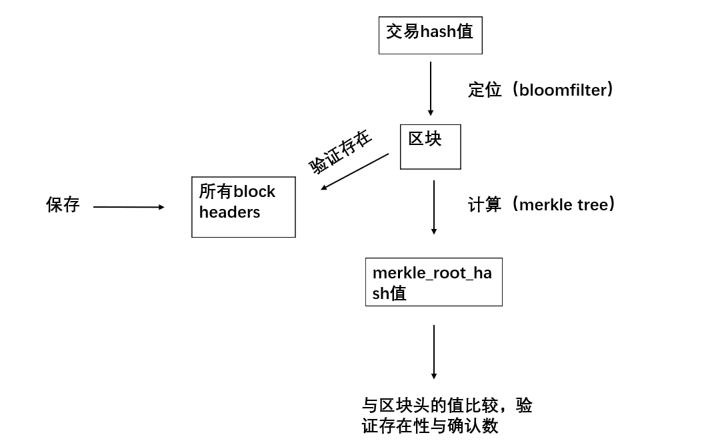
\includegraphics[width=.9\textwidth]{spv.png}
	\caption{spv验证流程}
\end{figure}

\subsubsection{SPV优化}

SPV在实现上涉及到一个问题:如何才能通过交易记录来定位到该资金转移所在的区块(上述流程第二步)。去中心方式下,为了定位block,客户端有时不得不下载整个区块链。

利用Bloom filter的方式,可解决区块检索的问题。Bloom Filter是一种空间效率很高的随机数据结构,它利用位数组很简洁地表示一个集合,可以快速判断出某检索值一定不存在于某个指定的集合。从而可以过滤掉大量无关数据,去中心化方式SPV查询提供必要的支持。

下面是bloom filter执行原理:

step1:初始状态时,Bloom Filter是一个包含m位的位数组,每一位都置为0。

step2:对于S=\{x1, x2,…,xn\}这样含n个元素的集合,使用k个相互独立的哈希函数,它们分别将集合中的每个元素映射到\{1,…,m\}的范围中。对任意一个元素x,第i个哈希函数映射的位置hi(x)就会被置为1(1≤i≤k)。   

step3:在判断y是否属于这个集合时,我们对y应用k次哈希函数,如果所有hi(y)的位置都是1(1≤i≤k),y是集合中的元素,否则就认为y不是集合中的元素。

\section{总结}

\section*{附件:项目建议书}
\end{document} 